\chapter{A look under the hood: \\ Our process}

\ds{Make sure we talk about continuous integration / git processes / etc}

The first step in removing unnecessary redundancy is identifying exactly what
that redundancy is and where it exists. To that end we need to understand what
each of our software artifacts is attempting to communicate, who their audience
is, and what information can be considered boilerplate versus system-specific.
Luckily, we have an excellent starting point thanks to the work of many smart
people - artifact templates.

Lots of work \ds{cite some people who did this} has been done to specify 
exactly what should be documented in a given artifact in an effort for 
standardization. Ironically, this has led to many different `standardized' 
templates. Through the examination of a number of different artifact templates, 
we have concluded they convey roughly the same overall information for a given 
artifact. Most differences are stylistic or related to content 
organization and naming conventions.

Once we understand our artifacts, we take a practical, example-driven approach
to identifying redundancy through the use of existing software system case
studies. For each of these case studies, we start by examining the source code
and existing software artifacts to understand exactly what problem they are
trying to solve. From there, we attempt to distill the system-specific knowledge
and generalize the boilerplate.

\section{A (very) brief introduction to our case study systems}
\ds{**NOTE: ensure each artifact has a 'who' (audience), 'what' (problem 
being solved), and 'how' (specific-knowledge vs boilerplate) - this last one 
may not be necessary}

To simplify the process of identifying redundancies and patterns, we have chosen
several case studies developed using common artifact templates, specifically 
those used by \smithea{} \ds{source?} Also, as mentioned in 
Section~\ref{sec:scope}, we have chosen software systems that follow the 
$`input' \rightarrow `process' \rightarrow `output'$ pattern. These systems 
cover a variety of use cases, to help avoid over-specializing into one 
particular system type. 

The majority of the aforementioned case studies were developed to solve real
problems. The following cards are meant to be used as a high-level reference to 
each case study, providing the general details at a glance. For the specifics 
of each system, all relevant case study artifacts can be found at \ds{Add a 
link here or put in appendices?}.

\card{\gb}
{We need to efficiently and correctly predict whether a glass 
slab can withstand a blast under given conditions.}
{\ds{TODO - Fill in once all examples in the thesis are done}}

\card{\sw}
{Solar water heating systems incorporating phase change 
 material (PCM) use a renewable energy source and provide a novel way of 
 storing energy. A system is needed to investigate the effect of employing PCM
 within a solar water heating tank.}
{\ds{TODO}}

\card{\np}
{Solar water heating systems provide a novel way of 
heating water and storing renewable energy. A system is needed to investigate
the heating of water within a solar water heating tank.}
{\ds{TODO}}

The NoPCM case study was created as a software family member for the SWHS case
study. It was manually written, removing all references to PCM and thus 
remodeling the system.

\card{\sp}
{A slope of geological mass, composed of soil and rock 
 and sometimes water, is subject to the influence of gravity on the mass. 
 This can cause instability in the form of soil or rock movement which can
 be hazardous. A system is needed to evaluate the factor of safety of 
 a slope's slip surface and identify the critical slip surface of the slope, 
 as well as the interslice normal force and shear force along the critical 
 slip surface.}
{\ds{TODO}}

\card{\pr}
{A system is needed to efficiently and correctly predict
 the landing position of a projectile.}
{\ds{TODO}}

The Projectile case study, was the first example of a system 
created solely in Drasil, i.e. we did not have a manually created version to 
compare and contrast with through development. As such, it will not be 
referenced often until \ds{DRASILSECTION} since it did not inform Drasil's 
design or development until much further in our process. The Projectile case 
study was created post-facto to provide a simple, understandable example for a 
general audience as it requires, at most, a high-school level understanding of 
physics. 

\card{\gp}
{Many video games need physics libraries that simulate 
 objects acting under various physical conditions, while simultaneously being 
 fast and efficient enough to work in soft real-time during the game. 
 Developing a physics library from scratch takes a long period of time and is 
 very costly, presenting barriers of entry which make it difficult for game 
 developers to include physics in their products.}
{\ds{TODO}}

After carefully selecting our case studies, we went about a practical approach
to find and remove redundancies. The first step was to break down each artifact
type and understand exactly what they are trying to convey.


\section{Breaking down \sfs}
\label{sec:breakdown}

As noted earlier, for our approach to work we must understand exactly what each
of our artifacts are trying to say and to whom.\footnote{Refer to 
Section~\ref{sec:sfs} for a general summary of \sfs{}.} By selecting our case 
studies from those developed using common artifact templates, we have given 
ourselves a head start on that process, however, there is still much work to be 
done.

\subsection{SRS}

To start, we look at the Software Requirements Specification (SRS). The SRS
(or some incarnation of it) is one of the most important artifacts for any
software project as it specifies what problem the software is trying to solve.
There are many ways to state this problem, and the template from \smithea{} has 
given us a strong starting point. Figure~\ref{fig:SRSToC} shows the table of 
contents for an SRS using the \smithea{} template.

\fig{
  \begin{center}
\footnotesize
\begin{enumerate}[nosep, label*=\arabic*.]
\item Reference Material
\begin{enumerate}[nosep, label*=\arabic*.]
  \item Table of Units
  \item Table of Symbols
  \item Abbreviations and Acronyms
\end{enumerate}
\item Introduction
\begin{enumerate}[nosep, label*=\arabic*.]
  \item Purpose of Document
  \item Scope of Requirements
  \item Characteristics of Intended Reader
  \item Organization of Document
\end{enumerate}
\item Stakeholders
\begin{enumerate}[nosep, label*=\arabic*.]
  \item The Customer
  \item The Client
\end{enumerate}
\item General System Description
\begin{enumerate}[nosep, label*=\arabic*.]
  \item System Context
  \item User Characteristics
  \item System Constraints
\end{enumerate}
\item Specific System Description
\begin{enumerate}[nosep, label*=\arabic*.]
  \item Problem Description
\begin{enumerate}[nosep, label*=\arabic*.]
    \item Physical System Description
    \item Goal Statements
\end{enumerate}
  \item Solution Characteristics Specification
\begin{enumerate}[nosep, label*=\arabic*.]
    \item Assumptions
    \item Theoretical Models
    \item General Definitions
    \item Data Definitions
    \item Instance Models
    \item Data Constraints
    \item Properties of a Correct Solution
\end{enumerate}
\end{enumerate}
\item Requirements
\begin{enumerate}[nosep, label*=\arabic*.]
  \item Functional Requirements
  \item Non-Functional Requirements         
\end{enumerate}
\item Likely Changes
\item Unlikely Changes
\item Traceability Matrices and Graphs
\item Values of Auxiliary Constants
\item References
\item Appendix
\end{enumerate}
  \end{center}
}{The Table of Contents from the (\ds{expanded?}) \smithea{} 
template}{fig:SRSToC}

With the structure of the document in mind, let us look at several of our case
studies' SRS documents to get a deeper understanding of what each section truly
represents. Figure~\ref{fig:csRefSecs} shows the reference section of the SRS 
for \gb. Each of the case studies' SRS contains a similar section so for 
brevity we will omit the others here, but they can be found at \ds{TODO}. 
% Provide a link / ref to relevant appendix
We will look into the case studies in more detail later, for now we will try to 
ignore any superficial differences (spelling, grammar, phrasing, etc.) in each 
of them while we look for commonality. We are also trying to determine how the 
non-superficial differences relate to the document template, general problem 
domain, and specific system information.

\fig{
\centering
%\emph{Figure showing the Ref Section of one case 
%			study, split into multiple subfigures - case study TBD}
\begin{subfigure}{\textwidth}
\centering
\fbox{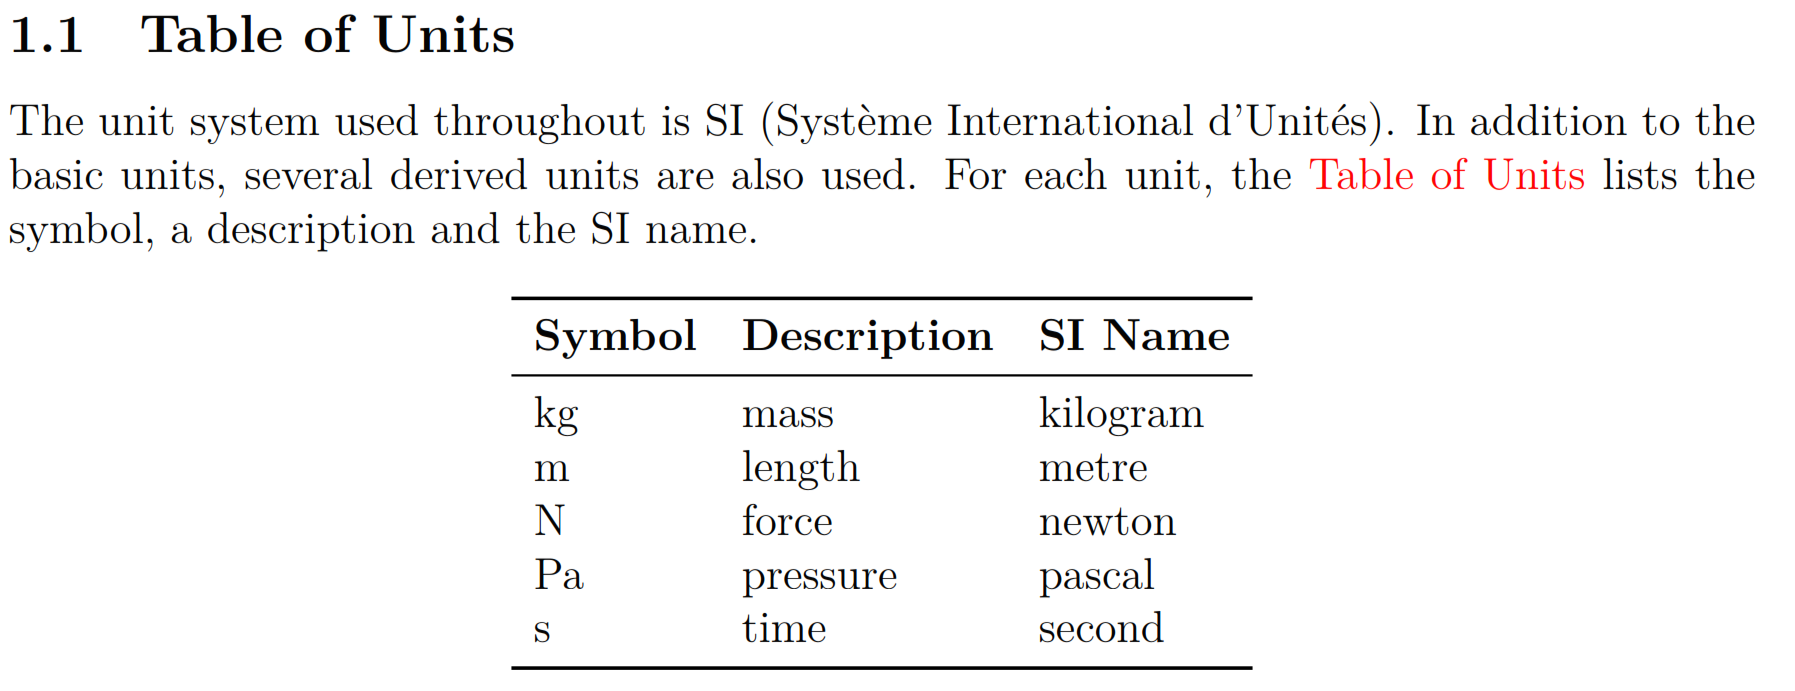
\includegraphics[width=\textwidth]{figures/gb_SRS_ToU.png}}
\caption{Table of Units Section}
\label{fig:gbrtou}
\end{subfigure}

\end{figure}

\begin{figure}\ContinuedFloat

\begin{subfigure}{\textwidth}
\centering
\fbox{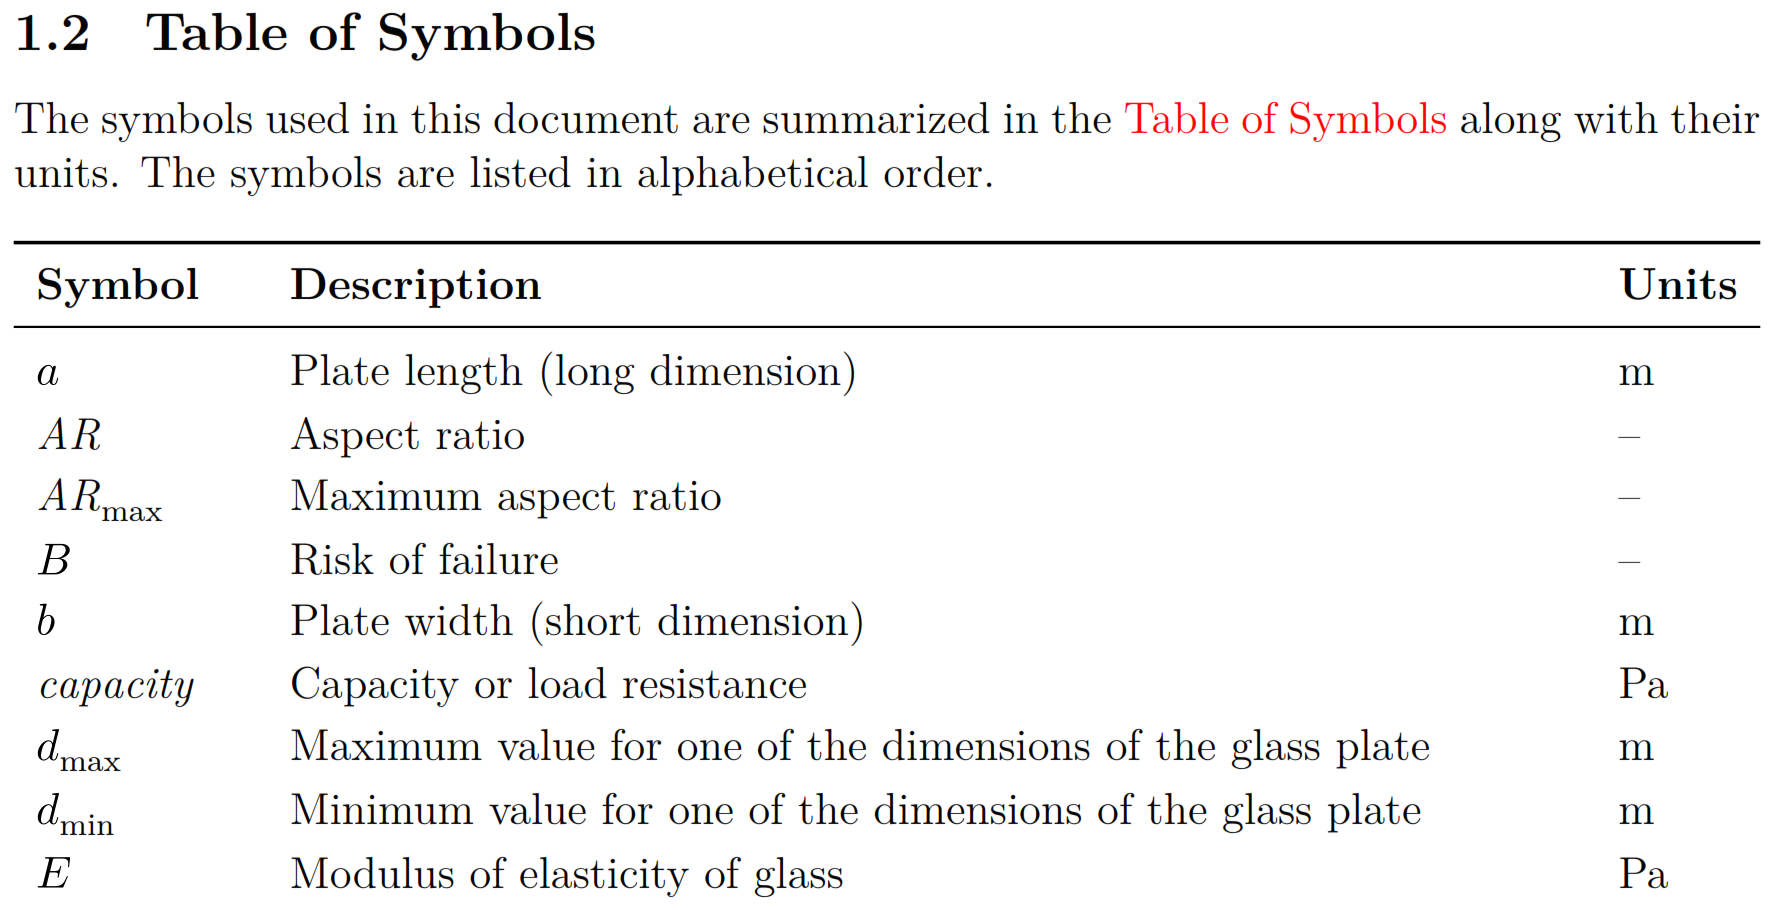
\includegraphics[width=\textwidth]{figures/gb_SRS_ToS.png}}
\caption{Table of Symbols (truncated) Section}
\label{fig:gbrtos}
\end{subfigure}


\begin{subfigure}{\textwidth}
\centering
\fbox{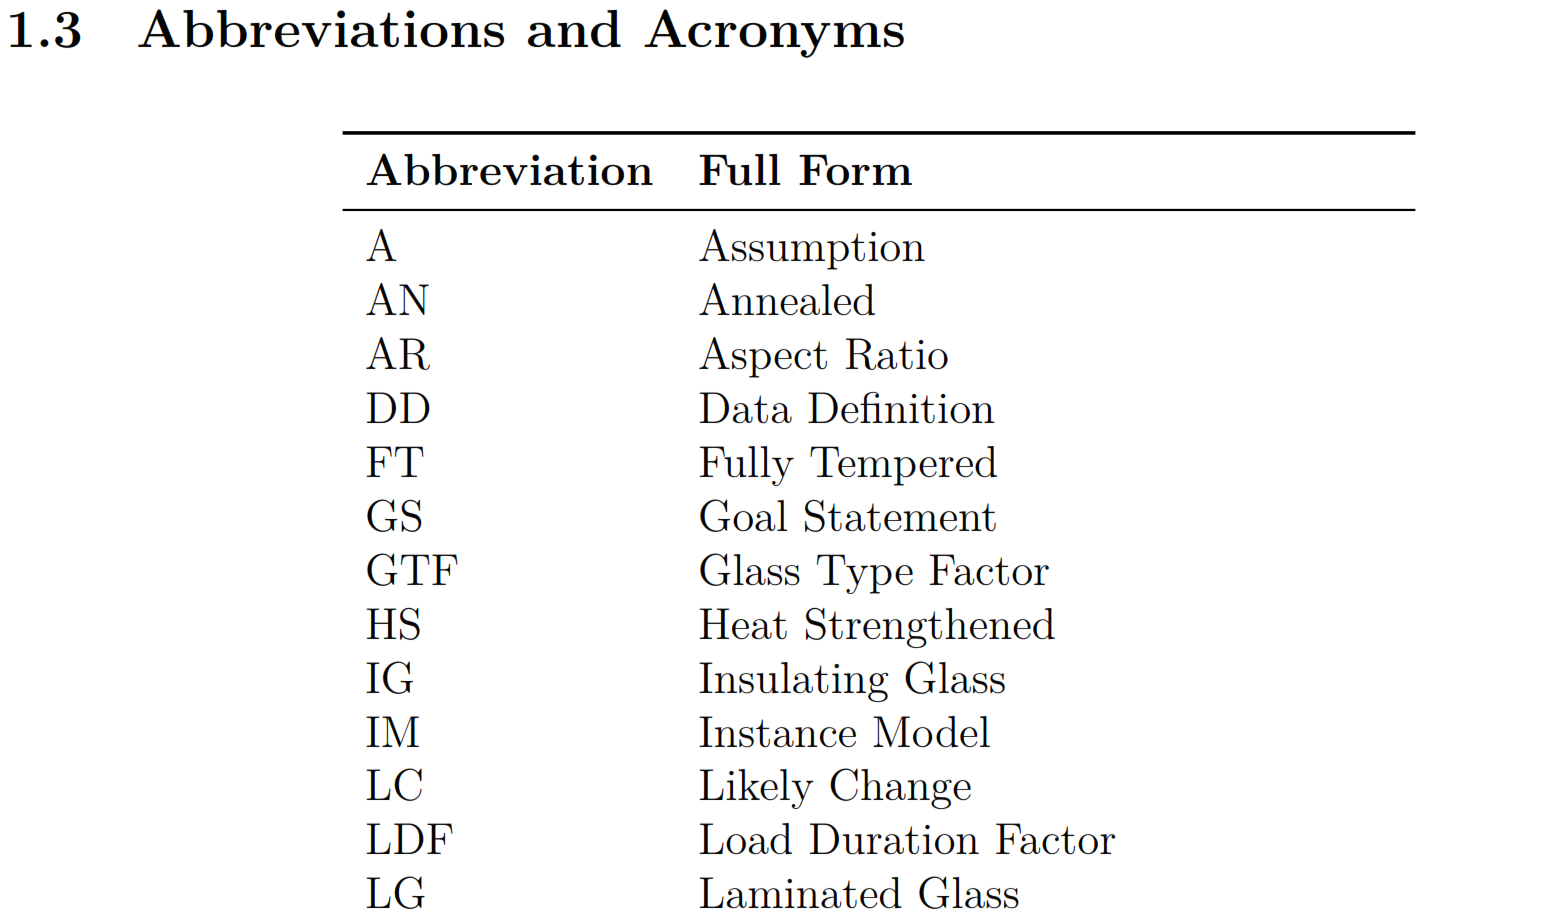
\includegraphics[width=\textwidth]{figures/gb_SRS_ToAA.png}}
\caption{Table of Abbreviations and Acronyms (truncated) Section}
\label{fig:gbrtoa}
\end{subfigure}
}
{The reference sections of \gb}
{fig:csRefSecs}

Looking at the (truncated for space) Table of Symbols, Table of Units, and 
Table of Abbreviations and Acronyms sections (Figure~\ref{fig:csRefSecs}) we 
can see that, barring the table values themselves, they are almost identical. 
The Table of Symbols is simply a table of values, akin to a glossary, specific 
to the symbols that appear throughout the rest of the document. For each of 
those symbols, we see the symbol itself, a brief description of what that 
symbol represents, and the units it is measured in, if applicable. Similarly, 
the Table of Units lists the Syst\`eme International d'Unit\'es (SI) Units used 
throughout the document, their descriptions, and the SI name. Finally, the 
table of Abbreviations and Acronyms lists the abbreviations and their full 
forms, which are essentially the symbols and their descriptions for each of the 
abbreviations.

While the reference material section should be fairly self-explanatory as to 
what it contains, other sections and subsections may not be so clear from their 
name alone. For example, it may not be clear offhand of what constitutes a 
theoretical model compared to a data definition or an instance model. One may 
argue that the author of the SRS, particularly if they chose to use the 
\smithea{} template, would need to understand that difference. However, it is 
not clear whether the intended audience would also have such an understanding. 
Who is that audience? Refer to Section~\ref{sec:sfs}, for more details. A brief 
summary is available in Table~\ref{tab:sfsummary}.

Returning to our exercise of breaking down each section of the SRS to determine 
the subtleties of \emph{what} is contained therein\footnote{The breakdown 
details are omitted for brevity and due to their monotonous nature, although 
the overall process is very much akin to the breakdown of the Reference 
Material section.} it should be unsurprising that each section maps to the 
definition provided in the \smithea{} template. However, as noted above, we can 
see distinct differences in the types of information contained in each section. 
Again we find some is boilerplate text meant to give a generic 
(non-system-specific) overview, some is specific to the proposed system, and 
some is in-between: it is specific to the problem domain for the proposed 
system, but not necessarily specific to the system itself.

Observing the contents of an SRS template adhere to said template may seem 
mundane, but it is a necessary step before we can move on to other \sfs{}. 
Without understanding what the SRS template intends to convey it is hard to 
assess weather or not the case study SRS conveys that information. With that in 
mind, we can move on to the MG and source code.

\ds{Current plan for following subsections: Brief description of the \sf{}, 
show an example of similarities within (ex. MG/MIS have a section per module, 
each section is organized the same way, some are filled in, some aren't), then 
follow a requirement through the MG to something in the MIS and finally to 
code. We'll dissect differences between case studies when looking at the 
patterns in Section~\ref{sec:patterns}. This also plants the seeds of "see, 
there's the same info moving from SRS $\rightarrow$ MG $\rightarrow$ MIS** 
$\rightarrow$ Code without stating it 
explicitly, which we can then do in the pattern section.}

\ds{Example to use should be a DD/IM from GlassBR, goes to calculations module 
in the MG, and finally a method in the source code}

\subsection{Module Guide}

The module guide (MG) is a \sf{} that details the architecture of a given 
software system. It holds a number of design decisions around sensibly grouping 
functionalities within the system into modules to fulfill the requirements laid 
out in the SRS. For example, one might have an input/output module for handling 
user input and giving the user feedback through the display (ie. via print 
commands or some other output), or a calculations module that contains all of 
the calculation functions being performed in the normal operation of the given 
software system. The \smithea{} MG template also includes a traceability matrix 
for ease of verifying which requirements are fulfilled by which modules.
Finally, the MG includes considerations for anticipated or unlikely changes 
that the system may undergo during its lifecycle.

\fig{
\begin{center}
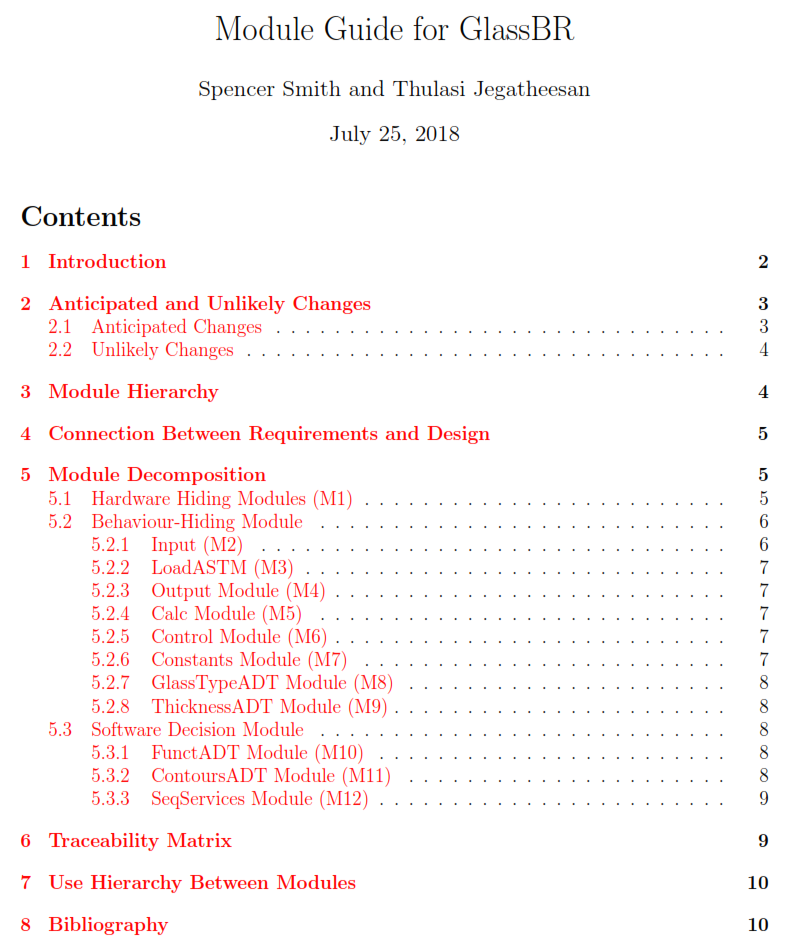
\includegraphics[width=\linewidth]{figures/gb_MG_ToC.png}
\end{center}}
{Table of Contents for GlassBR Module Guide}
{fig:gbrmgtoc}

Figure~\ref{fig:gbrmgtoc} shows the table of contents for the \gb{} case 
study's MG. For the sake of brevity we will omit the other case studies 
here (they can be found at \ds{TODO}). Just as with the SRS we are looking for 
commonality and understanding of what the document is trying to portray to the 
reader. As such we will ignore superficial differences between the MG sections. 
As the MG is a fairly short document we will look at each of the most relevant 
sections as part of this exercise.

Breaking down the MG by section, we can see that the introduction is itself 
completely generic boilerplate explaining the purpose of the MG, the audience, 
and some references to other works that explain why we would make certain 
choices over other (reasonable) ones given the opportunity. There is nothing 
system-specific, nor specific to the given problem domain of the case study.

Following through the table of contents into the ``Anticipated and Unlikely 
Changes" section, we see that again the introductions to this section and 
its subsections are generic boilerplate, however the details of each section 
are not. Both subsections are written in the same way: as a list of labeled 
changes (AC\# for anticipated change, UC\# for unlikely change). This is the 
first place we see both problem-domain and system specific information 
Interestingly, the Module Hierarchy section follows the same general style: it 
is a list of modules which represent the leaves of the module hierarchy tree 
and each one is labeled (M\#).

\fig{
\begin{center}
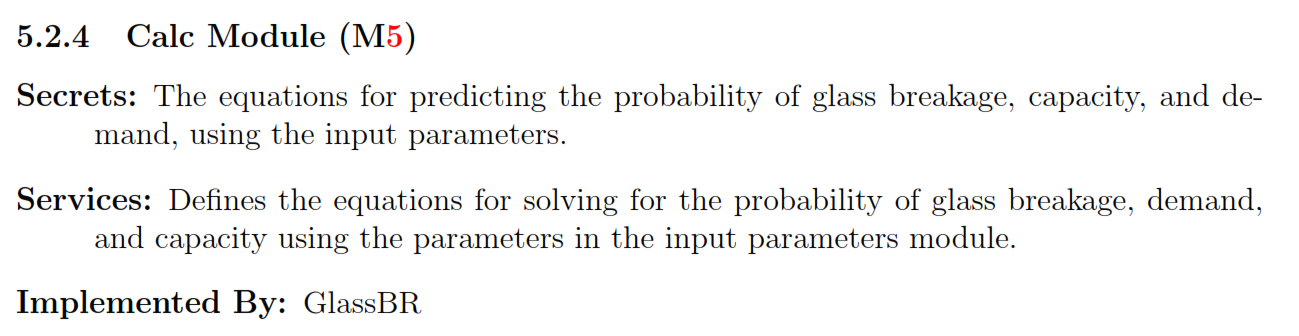
\includegraphics[width=\linewidth]{figures/gb_MG_CM.png}
\end{center}}
{Calc Module from the \gb{} Module Guide}
{fig:gbrmgcm}

Skipping ahead to the module decomposition, we find a section heading for each 
Level 1 module in the hierarchy, followed by subsections describing the Level 2 
modules. The former are almost entirely generic boilerplate (for example common 
Level 1 modules include: Hardware-Hiding, Behaviour-Hiding, and 
Software Decision modules), but the latter are problem-domain or system 
specific. An example of a system-specific module is shown in 
Figure~\ref{fig:gbrmgcm}. 

Each module is described by its secrets, services, and what it will be 
implemented by. For example, a given module could be implemented by the 
operating system (OS), the system being described (ex. \gb{}), or a third party 
system/library that will inter-operate with the given system.

Finally we have a traceability matrix and use hierarchy diagram. Both are 
visual representations of how the different modules implement the requirements 
and use each other respectively. The traceability matrix provides a direct and 
obvious link between the SRS and MG, where other connections between the two 
\sfs{} have been implicit until this point. Generally, the next \sf{} would be 
the MIS, however as it is structured so similarly to the MG (one section per 
module, each section organized in a very similar way, a repeated use hierarchy, 
etc) we will skip it for brevity. The MIS includes novel system-specific, 
implementation-level information denoting the interfaces between modules, but 
for our exercise does not provide any revelations beyond that of the MG.

The MG gives us a very clear picture of \textit{decisions} made by the system 
designers, as opposed to the knowledge of the system domain, problem being 
solved, and requirements of an acceptable solution provided in the SRS. The MG 
provides platform and implementation-specific decisions, which will eventually 
be translated into implementation details in the source code. With that in 
mind, let us move on to the source code.

\subsection{Source Code}

The source code is arguably the most important \sf{} in any given software 
system as it serves as the set of instructions that the computer executes in 
order to solve the given problem. With only the other \sfs{} and without the 
source code, we would have a very well defined problem and solution criteria, 
but would never solve the problem.

\fig{
\begin{center}

\begin{forest}
  for tree={
    font=\ttfamily,
    grow'=0,
    child anchor=west,
    parent anchor=south,
    anchor=west,
    calign=first,
    edge path={
      \noexpand\path [draw, \forestoption{edge}]
      (!u.south west) +(7.5pt,0) |- node[fill,inner sep=1.25pt] {} (.child 
      anchor)\forestoption{edge label};
    },
    before typesetting nodes={
      if n=1
        {insert before={[,phantom]}}
        {}
    },
    fit=band,
    before computing xy={l=25pt},
  }
[/src/Python
  [Calc.py]
  [Constants.py]
  [ContoursADT.py]
  [Control.py]
  [Exceptions.py]
  [FunctADT.py]
  [GlassTypeADT.py]
  [Input.py]
  [LoadASTM.py]
  [Output.py]
  [SeqServices.py]
  [ThicknessADT.py]
]
\end{forest}

\end{center}
}
{Python source code directory structure for \gb{}}
{fig:gbsrcstruct}

As the source code is the executable set of instructions for a system to solve 
a problem, one would expect it to be almost entirely system and problem-domain 
specific with very little boilerplate. Looking into the source of our case 
studies, we find this to be mostly true barring the most generic of library use 
(ex. \lstinline[language=C]|stdio| in C).

Returning to our example of the MG from \gb{} (Figure~\ref{fig:gbrmgtoc}) and 
comparing it to the python source code structure shown in 
Figure~\ref{fig:gbsrcstruct} we can see that the source code follows almost 
identically in structure to the module decomposition. The only difference is 
that we also observe an exceptions module defining the different varieties of 
exceptions that will be thrown by the other modules. While this is a fairly 
trivial difference, likely made for ease of maintenance, readability, and 
extensibility, it highlights this fairly obvious difference between the two 
\sfs{}. A difference which we speculate was caused by a change made during the 
implementation phase where the MG was not updated to reflect the addition of an 
exceptions module.



\section{Patterns and repetition and patterns and repetition -- (OR -- 
Repeating patterns and patterns that repeat --)}
\label{sec:patterns}
  \ds{\sout{**Make sure to mention "We actually found that some
  info is boilerplate, some is system-specific, and some is general to all
  members of a software family, but more specific than generic boilerplate"}}
\ds{Pretty sure I got that covered earlier}

\ds{This part isn't exactly true with the reorg of info. I'm going to show some 
patterns here instead}. \sout{From the above sections, we see many emerging 
patterns 
in our \sfs{}. Ignoring, 
for now, the organizational patterns from the \smithea{} templates we can 
already see simple patterns emerging.}

Returning to our example from Section~\ref{sec:breakdown}, looking only at the 
reference section of our SRS template, we have already found
three subsections that contain the majority of their information in the same
organizational structure: a table of symbols and general information relevant 
to those symbols. Additionally, we can see that the Table of Units and Table of 
Symbols have an introductory blurb preceding the tables themselves, whereas the 
Table of Abbreviations and Acronyms does not. Inspecting across case studies, 
we can see that the introduction to the Table of Units is simply boilerplate 
text dropped into each case study verbatim, thus is completely generic and 
applicable to \emph{any} software system using SI units. The introduction to 
the Table of Symbols appears to be boilerplate across several examples, 
however, it does have some variation which we can see by comparing 
Figure~\ref{fig:gbrtos} to Figure~\ref{fig:gptos} (\gb{} compared to \gp{}).
These variations reveal the obvious: the variability between systems is greater 
than simply a difference in choice of symbols, and so there is some 
system-specific knowledge being encoded. We can intuit this conclusion based 
solely on each system solving a different problem, however, we have confirmed 
this by solely looking at the structure (patterns) of one section of the SRS.

\fig{
\centering
\fbox{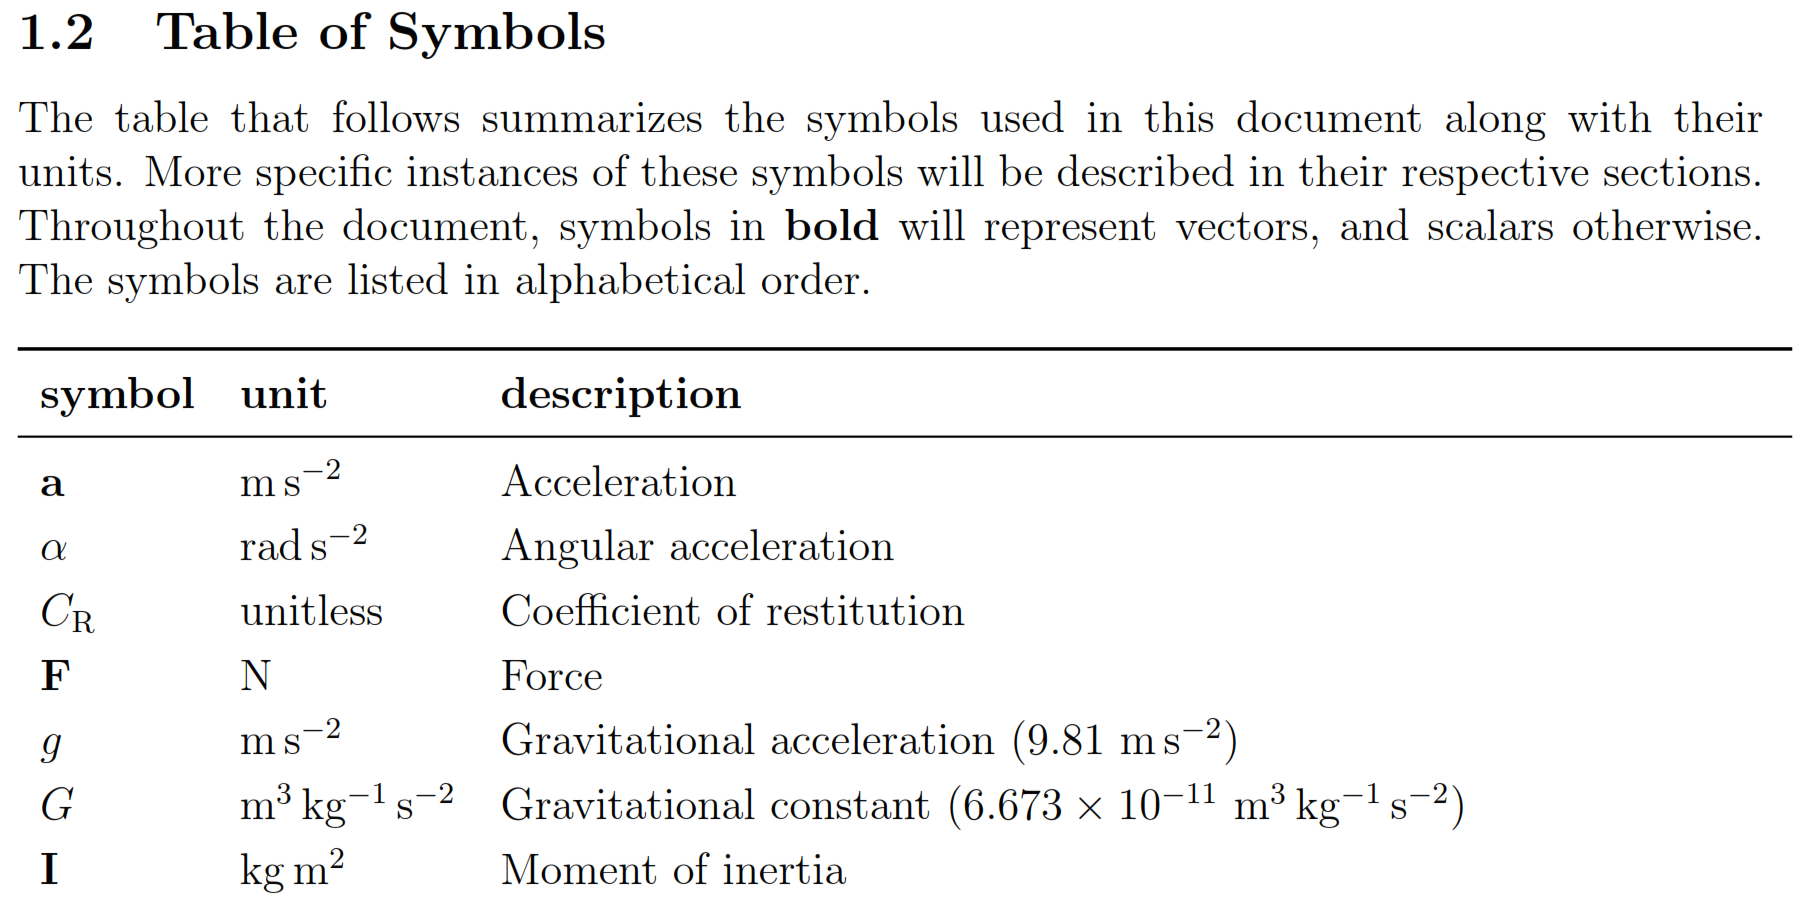
\includegraphics[width=\textwidth]{figures/gp_SRS_ToS.png}}
}
{Table of Symbols (truncated) Section from \gp{}}
{fig:gptos}

The reference section of the SRS provides a lot of knowledge in a very 
straightforward and organized manner. The basic units provided in the table of 
units give a prime example of fundamental, global knowledge shared across 
domains. Nearly any system involving physical quantities will use some of these 
units. On the other hand, the table of symbols provides system/problem-domain 
specific knowledge that will not be useful across unrelated domains. For 
example, the stress distribution factor $J$ from GlassBR may appear in several 
related problems, but would be unlikely to be seen in something like SWHS, 
NoPCM, or Projectile. Finally, acronyms are very context-dependent. They are 
often specific to a given domain and, without a coinciding definition, it can 
be very difficult for even the target audience to understand what they refer 
to. Within one domain, there may be several acronyms meaning different things, 
for example: PM can refer to Product Manager, Project Manager, Program 
Manager, etc.

By continuing to breakdown the SRS and other \sfs{}, we are able to find many 
more patterns. For example, we see the same concept being introduced in 
multiple areas within a single artifact and across artifacts in a project. 
\ds{Example from one of the figures in the previous section. Preferably 
something like a DD or TM that shows up within a single doc multiple times}. We 
also see patterns of commonality across software family members (The SWHS and 
NoPCM case studies) as they have been developed to solve similar, or in our 
case nearly identical, problems.

- inter-project (repetition throughout different views + other patterns.)
  vs intra-project knowledge (repetition across projects/family members,
  minor modifications, but fundamentally the same + other patterns.)
- Hint at chunkifying/parceling out the fundamental (system/view-agnostic)
knowledge vs the specific knowledge

\ds{Need to talk about knowledge projection/transformation in this section
- Use a relevant example from Case studies, maybe from PCM? Something like 
$\Delta{}U = Q - W$ is the same as ``Total energy within a closed system must 
be conserved" but transformed for / projects out what is relevant to a given 
audience.
- This will be useful for the following section}

\section{Organizing knowledge - a fluid approach}
  **Subsec roadmap:
    - We see the patterns above, we can generalize a lot of that
    - Direct repetition (copy-paste) vs indirect repetition (view-changes)
    require us to pull together knowledge from all artifacts into one place
    - Some can be derived automatically, the rest must be explicitly stated
    - We need to create a categorization system (hint at chunks) that is both
    robust and extensible to cover a wide variety of use cases.
    - Finally the templates give us structure

  **NOTE: Under the hood section should explain the process of how we determined
  what we needed to do. What we ended up doing should come in the following
  section(s) - no 'real' implementation details, only conceptual stuff here.
  
\section{The seeds of Drasil}
  **Subsec roadmap:
    -- Summarize the above subsections and lead into next section
    -- Add relevant information that doesn't quite fit above 
      and isn't implementation related
    -- 'Relevant buckshot section'